% turbo-user-guide.tex
% PJ, October 2011
%
\documentclass[12pt,a4paper,twoside]{article}
\usepackage[body={16cm,24.5cm}]{geometry}
\usepackage{hyperref}
\hypersetup{colorlinks=true,linkcolor=blue}
\usepackage{graphicx}
\usepackage{makeidx}
% \usepackage{showidx}
\usepackage{listings}
\usepackage{lscape}
\usepackage{longtable}
\lstset{basicstyle=\ttfamily\scriptsize,identifierstyle=,keywordstyle=}
\usepackage{amsmath}
\usepackage{amssymb}

%------------------------------------------------------------------
% a couple horizontal bars to delimit embedded code
% the width suits the page size set above and
% the mathmode eliminates spaces between the three elements
\newcommand{\topbar}{\ensuremath{
    \rule{0.1mm}{2.0mm} \rule[2.0mm]{159.5mm}{0.1mm} \rule{0.1mm}{2.0mm}
}}
\newcommand{\bottombar}{\ensuremath{
    \rule{0.1mm}{2.0mm} \rule{159.5mm}{0.1mm} \rule{0.1mm}{2.0mm}
}}
\newcommand{\topbarshort}{\ensuremath{
    \rule{0.1mm}{2.0mm} \rule[2.0mm]{149.5mm}{0.1mm} \rule{0.1mm}{2.0mm}
}}
\newcommand{\bottombarshort}{\ensuremath{
    \rule{0.1mm}{2.0mm} \rule{149.5mm}{0.1mm} \rule{0.1mm}{2.0mm}
}}
%------------------------------------------------------------------

\title{
    Turbine Simulations with Eilmer3.
}
\author{
    Mechanical Engineering Report 2011/xx\\
    Peter Jacobs, Paul Petrie-Repar, Carlos de Miranda-Ventura,\\
    Emilie Sauret, Jason Czapla, Peter Blyton,\\
    Haiko Rijkers\thanks{University of Twente, Netherlands} and 
    Paul van der Laan\thanks{University of Twente, Netherlands},\\
    Queensland Geothermal Energy Centre of Excellence,\\
    The University of Queensland, Brisbane, Australia.
} 
\date{October 2011}
\makeindex

\begin{document}
\maketitle

\begin{abstract}
In order to perform simulations of turbomachinery flow paths.
the in-house compressible-flow simulation code, \textit{Eilmer3}, 
has been adapted.
Specific adaptations include the addition of terms for the rotating frame of reference, 
programmable boundary conditions for periodic boundaries 
and a mixing plane interface between the rotating and non-rotating blocks.

\medskip
Simulations of various turbomachines using Eilmer3 then compared to 
reference calculations and experimental data to demonstrate it effectiveness
for turbomachinery calculations.
\end{abstract}

\cleardoublepage
\tableofcontents

%------------------------------------------------------------------
\cleardoublepage
\baselineskip = 1.5pc

\section{Introduction}
\label{intro-sec}
%
Our in-house code, \textit{Eilmer3}, has been developed over the past few years 
for the simulation of hypersonic flows.
Being built specifically to model the flow in shock and expansion tubes,
it solves the compressible Navier--Stokes equations via a cell-centred time-dependent finite-volume formulation.
The governing equations are expressed in integral form over arbitrary hexahedral cells, 
with the time rate of change of conserved quantities in each cell specified as a summation of 
the mass, momentum and energy flux through the cell interfaces.  
The code has come from a hypersonics research background is also specialised 
for simulating flows in 2D axisymmetric geometries.
The thermochemistry module can handle gases in chemical equilibrium or nonequilibrium.
When simulating gases with finite-rate chemistry and radiation energy exchange, 
these physical processes are treated with an operator-split approach. 
The computational core of \textit{Eilmer3} is written in a combination of C and C++, 
with the option for user-defined functions such as boundary conditions provided as Lua scripts.
Preprocessing (\textit{i.e.} grid generation) and postprocessing is handled by a collection of Python programs.

\medskip
For a more detailed description of the numerical methods coded into \texttt{Eilmer3}, 
see the companion report \cite{jacobs_etal_2010b}
which covers the gas-dynamic formulation and the basic thermochemistry components.

\cleardoublepage

\section{The code}

\subsection{Gas-Dynamic Formulation}
\label{formulation-sec}
%
The code is formulated around the integral form of the Navier-Stokes equations, which can be expressed as
\begin{equation}
 \frac{\partial}{\partial t} \int_{V} U dV = - \oint_{S} \left ( \overline{F}_{i} - \overline{F}_{v} \right ) \cdot \hat{n}~dA + \int_{V} Q dV \text{ , }
 \label{eq:NS}
\end{equation}
where $S$ is the bounding surface and $\hat{n}$ is the outward-facing unit normal of the control surface.
Two-dimensional and three-dimensional formulations are implemented somewhat separately in \textit{Eilmer3},
however, there is much of the formulation and code that is the same for both cases. 
Considering a single-species gas, the vector of conserved quantities can be written as
\begin{equation}
 U = \left [ \begin{array}{c} \rho \\ 
                              \rho u_{x} \\ 
                              \rho u_{y} \\ 
                              \rho u_{z} \\ 
                              \rho E
             \end{array} \right ] \text{ . }
 \label{eq:U_vector_3D}
\end{equation}
Here, the conserved quantities are respectively density, $x, y, z$-momentum per volume and total energy per volume.
For a rotating frame of reference, we choose the rotation to occur about the $z$-axis and follow the 
description in Ref.\,\cite{hirsch_2007a}. 
The relative velocity, $\vec{u}$, in the rotating frame is related to the intertial-frame velocity, $\vec{v}$,
as $\vec{v} = \vec{u} + \omega_z (x \hat{j} - y \hat{i})$, where $\omega_z$ is the angular speed of the frame.
The total energy is constructed as $E = e + \frac{1}{2} |\vec{u}|^2 - \frac{1}{2} \omega_z^2 r^2$, 
where $e$ is the specific internal energy and $r^2 = x^2 + y^2$, $r$ being the radial distance from the $z$-axis.

The inviscid component of the flux vector is
\begin{equation}
 \overline{F}_{i} = \left [ \begin{array}{c}
                               \rho u_{x} \\
                               \rho u_{x}^{2} + p \\
                               \rho u_{y} u_{x} \\
                               \rho u_{z} u_{x} \\
                               \rho E u_{x} + p u_{x}
                            \end{array} \right ] \hat{i} 
                  + \left [ \begin{array}{c} 
                               \rho u_{y} \\
                               \rho u_{x} u_{y} \\
                               \rho u_{y}^{2} + p \\
                               \rho u_{z} u_{y} \\
                               \rho E u_{y} + p u_{y}
                            \end{array} \right ] \hat{j} 
                  + \left [ \begin{array}{c} 
                               \rho u_{z} \\
                               \rho u_{z} u_{x} \\
                               \rho u_{z} u_{y} \\
                               \rho u_{z}^{2} + p \\
                               \rho E u_{z} + p u_{z}
                            \end{array} \right ] \hat{k} 
                 \text{ . }
 \label{eq:F_i_3D}
\end{equation}
The viscous component is
\begin{eqnarray}
 \overline{F}_{v} & = & \left [ 
                            \begin{array}{c} 
                                0 \\
                                \tau_{xx} \\
                                \tau_{yx} \\
                                \tau_{zx} \\
                                \tau_{xx} u_{x} + \tau_{yx} u_{y} + \tau_{zx} u_{z} + q_{x}
                            \end{array}
                          \right ] \hat{i} 
                        + \left [ 
                             \begin{array}{c}
                                 0 \\
                                 \tau_{xy} \\
                                 \tau_{yy} \\
                                 \tau_{zy} \\
                                 \tau_{xy} u_{x} + \tau_{yy} u_{y} + \tau_{zy} u_{z} + q_{y}
                             \end{array}
                          \right ] \hat{j}  + \nonumber \\
                  &   &   \left [
                             \begin{array}{c}
                                 0 \\
                                 \tau_{xz} \\
                                 \tau_{yz} \\
                                 \tau_{zz} \\
                                 \tau_{xz} u_{x} + \tau_{yz} u_{y} + \tau_{zz} u_{z} + q_{z}
                             \end{array}
                          \right ] \hat{k} \text{ , }
 \label{eq:F_v_3D}
\end{eqnarray}
and the viscous stresses are evaluated on the usual gradients of velocity.

The finite-volume cells are hexahedral with 6 (possibly-nonplanar) quadrilateral surfaces interfacing the
neighbouring cells.
Flux values are estimated at midpoints of the cell interfaces and  
the integral conservation equation (\ref{eq:NS}) is approximated as the algebraic expression
\begin{equation}
 \frac{dU}{dt} = - \frac{1}{V} \sum_{cell-surface} \left ( \overline{F}_{i} - \overline{F}_{v} \right ) \cdot \hat{n} \, dA + Q \text{ , }
 \label{eq:dUdt}
\end{equation}
where $U$ and $Q$ now represent cell-average values of the conserved-quantity vector and the source vector, respectively. 
The centrifugal and Coriolis forces are included in the source vector as
\begin{equation}
 Q = \left [ 
       \begin{array}{c} 
         0 \\
         \rho (+2 \omega_z u_y + \omega_z^2 x) \\
         \rho (-2 \omega_z u_x + \omega_z^2 y) \\
         0 \\
         0
       \end{array}
     \right ] \text{ . }
 \label{eq:Q_geom}
\end{equation}

\subsection{Grid and Boundary Conditions}
%
The flow domain is discretised as a set of structured, body-fitted grids.
Data arrays for each block are dimensioned such that
there is a buffer region, two cells deep, around the \textit{active cells},
which completely defines the flow domain covered by the block.
The buffer region contains \textit{ghost cells} which are used to hold a copy of the flow information
from adjacent blocks or to implement the boundary conditions.

For a boundary common to two blocks, the ghost cells in the
buffer region of each block overlap the active cells of the adjacent block.
The only interaction that occurs between blocks is the 
exchange of boundary data, prior to the reconstruction phase of each time step.
For the \textit{shared memory} version of the code, 
the exchange of cell-average data along the block boundaries takes place as
a direct copy from the active-cell of one block to the ghost-cell of the other block.
Thus, the cells along the common boundary of each block must match in both number and position.
Some logic is used within the exchange routines to set the appropriate indexing direction for each boundary.
The information on the connections between block boundaries is stored in a (global) connectivity array.
For each boundary on each block, this array stores the
identity of the adjacent block and the name of the connecting boundary on the adjacent block.

The inviscid-component of applied boundary conditions is implemented by also filling in 
the ghost-cell data and then applying the normal reconstruction and flux calculation without
further discrimination of the boundary cells.
This approach covers solid/slip walls, inflow and outflow boundaries.

For viscous simulations, boundaries may also be assigned as fixed temperature, 
no-slip or catalytic (chemical equilibrium at wall gas state) boundary conditions.
Such viscous boundary conditions also use data specified at the cell interfaces
that lie along the boundary surface.
These data are used in the derivative calculations that subsequently feed into 
the viscous fluxes.

The primary data held by the code are cell-average data, associated with cell centres.
To get the fluxes at cell interfaces, a variable-by-variable reconstruction is made of the flow field.
This is done in a one-dimensional fashion, working along one-index direction at a time.
\textit{Left} and \textit{Right} values of a flow variable at a cell interface
are evaluated as the corresponding cell average value plus a limited higher-order interpolated increment.
This is essentially a piecewise-parabolic reconstruction of the flowfield data.
For flows without strong compressions or shocks, 
\textit{Eilmer3} then uses a modified AUSMDV calculator~\cite{wada_liou_94a},
as described in Ref.\cite{jacobs_etal_2010b}.
Prior to applying the flux calculator at each interface, 
the velocity field is rotated into a coordinate system local to the cell interface, 
and after, that flux transformed back into the global coordinate system.

\subsection{Mixing-Plane Interface}
%
The stator-rotor interaction was modelled making use of a \textit{mixing plane} (MP) model \cite{Denton_1979}. 
Other authors (\cite{Barr_2009},\cite{Qiu_2009}, \cite{Li_2006}) used this approach to model the interaction between the bladed segments of radial turbines.
Contrasting with the \textit{multi-reference frame} (MRF) model \cite{Luo_1994}, this latter model (MP) is applicable when the flow at the interface between stationary and moving zones is not uniform and therefore represents a more suitable choice when modelling cases where a strong interaction between the stationary and rotating zones exists (i.e. current case). 
When following this approach, each zone is regarded as a steady state problem, taking the flow data from both the stator and rotor interface cells and averaging it. 
This removes any unsteadiness that could occur in the flow field between passages. 
This also requires less computational effort when compared to the sliding mesh model since its calculations are unsteady and also as a consequence of a higher number of blade passages needed when using this latter model to simulate cases with different number of blades between each blade row.
Presently, we have implemented the \textit{MP} interface to model the stator-rotor interaction.

Within \texttt{Eilmer3} here are also boundary conditions that allow the user 
to specify the ghost-cell data and boundary interface data via user-written functions.
These functions may also be used to bypass the internal flux calculators and specify the boundary
fluxes directly.
As described in Ref.\,\cite{van_der_Laan_2009} and shown in Appendix\,\ref{user-defined-bc-sec} 
for the Kofsky radial-inflow turbine example, 
these user-defined boundary conditions are used to implement:
\begin{itemize}
 \item the mixing-plane interface between the rotating and non-rotating blocks;
 \item the circumferentially-periodic boundary connecting segments of the volute,
    the gap between stator and rotor, and the segments of the diffuser;
 \item the subsonic inflow and outflow conditions.
\end{itemize}
The Wilcox-2006 $k-\omega$ turbulence model is available in the code but has not been exercised 
for the turbomachinery calculations thus far.

\cleardoublepage
%--------------------------------------------------------------------

\section{Kofsky Radial-Inflow Turbine}
\label{sec:kofsky_example}
%
For radial-inflow turbines, the availability of fully defined test cases in terms of geometry as well as operating conditions and experimental results was found to be scarce.
Therefore, this work will allow to set a standard test case for our code development and testing.
In this context, a small 10\,kW shaft output turbine tested by \textit{NASA}\,\cite{Kofskey_1966} was considered one of the most suitable sample cases since it was found to provide sufficient detail with respect to the overall test case (geometry and operating conditions). 
Experimental results regarding the turbine performance for two values of Reynolds number, considering both argon and air as the working fluids as well as different inlet conditions were also presented.
The design point values mentioned in Ref.\,\cite{Kofskey_1966} allowed the definition of the input conditions to be used
when considering using argon as the working fluid (see Table \ref{Table_Kofskey_Input_Conditions}).

\begin{table}[htbp]
  \begin{center}
      \begin{tabular}{|l|r|}
      \hline
      Total Mass Flow Rate [kg/s]  & 0.277  \\
      Total Inlet Pressure [kPa]   & 91     \\
      Total Inlet Temperature [K]  & 1083.3 \\
      Static Outlet Pressure [kPa] & 56.4   \\ 
      Inlet Flow Angle [deg]       & 55.6   \\
      Rotational Speed [RPM]       & 38500  \\
      \hline
    \end{tabular}
  \end{center}
  \vskip-.4cm
  \caption{Flow Conditions used as Boundary Conditions for both \textit{CFX} and \textit{Fluent} with argon as the working fluid.}
  \vskip-.4cm
  \label{Table_Kofskey_Input_Conditions}
\end{table}

\subsection{Geometric model}
\label{sec:kofsky_geometry}
%
A simplified three-dimensional geometry of the \textit{NASA} turbine was also considered. For this case, the procedure reported by Krijgsman\,\cite{Krijgsman_2008} was followed, considering both the stator and rotor and assuming an infinitesimal blade thickness as well as no clearances for both the stator vanes and rotor blades.

In Krijgsman's work, several steady state simulations were carried out using \textit{Fluent} considering different approaches such as inviscid/viscous rotor analysis as well as different stator-rotor interaction models. 
An off-design performance evaluation was carried out by comparing the results against experimental data reported in Ref.\,\cite{Kofskey_1966} when considering several pressure-ratios, maintaining the total inlet pressure and changing the mass flow rate. 
Krijgsman's results showed good agreement with the \textit{NASA} values\,\cite{Kofskey_1966} but the assumed stator inlet flow angles were found to deviate from the reported inlet conditions. 
Therefore, the input conditions presented in Table~\ref{Table_Kofskey_Input_Conditions} were used for the current calculations 
and further tests (not shown in this paper) were performed to explore the influence of the input flow angles.
Relative to Krijgsman's results, the new tests showed a difference of 5.45\% and 6.50\% for both the total-total efficiency and total-static efficiency respectively as well as a 1.2\% difference in terms of power output.

Approximate three-dimensional geometries were also defined making use of commercial radial-inflow turbine design software packages \textit{RITAL} and \textit{AxCent} from \textit{Concepts NREC} (\texttt{http://www.conceptsnrec.com}). 
These geometries were re-created by optimising the one-dimensional preliminary design obtained with \textit{RITAL} in order to obtain a similar design as well as similar velocity triangles and using these results to create suitable three-dimensional geometries from \textit{AxCent}. 
Two fully-defined three-dimensional geometries were obtained from \textit{AxCent}. Both geometries take into account a pre-set blade thickness distribution and the main difference between these cases is the absence and presence of (blade-shroud) clearances respectively.
The one-dimensional analysis results compared with the \textit{NASA} reported data are presented in Table \ref{Table_Comparison_RITAL_NASA}. 

\begin{table}[htbp]
  \begin{center}
    \begin{tabular}{*{4}{|c}|}
      \hline
      & \textit{NASA} & \textit{RITAL} & Error [\%] \\
      & reported      & computed       &            \\
      \hline
      \hline
      Inlet Stator &  &  & \\
      \hline
      $\alpha$ [deg] & 55.60 & 55.40 & 0.36 \\
      C [m/s] & 107.35 & 109.45 & 1.95 \\
      \hline
      \hline
      Outlet Stator &  &  & \\
      \hline
      $\alpha$ [deg] & 72.00 & 72.35 & 0.49 \\
      C [m/s] & 288.05 & 280.80 & 2.50 \\ 
      \hline
      \hline
      Inlet Rotor & & & \\
      \hline
      $\alpha$ [deg] & 71.80 & 72.30 & 0.70 \\
      $\beta$ [deg] & -23.60 & -21.20 & 10.17 \\
      C [m/s] &  283.30 & 287.00 & 1.31 \\
      W [m/s] & 96.50 & 94.10 & 2.49 \\
      \hline
      \hline
      Outlet Rotor & & & \\
      \hline
      $\alpha$ [deg] & 10.20 & 12.20 & 19.61 \\
      $\beta$ [deg] & -50.80 & -50.80 & set \\
      C [m/s] & 148.80 & 116.80 & 21.51 \\
      W [m/s] & 231.70 & 180.60 & 22.05\\
      \hline
      \hline
      $\eta_{t-t}$ & 0.880  & 0.877 & 0.34 \\
      $\eta_{t-s}$ & 0.824 & 0.817 & 0.85  \\
      \hline
      \hline
      Total Power [kW] & 22.39  & 22.24 & 0.67 \\
      \hline
    \end{tabular}
  \end{center}
  \vskip-.4cm
  \caption{Comparison of \textit{RITAL} computational results and reported data from Ref.\,\cite{Kofskey_1966}.}
  \vskip-.4cm
  \label{Table_Comparison_RITAL_NASA}
\end{table}

The results are in fair agreement with the reported values, despite the differences in velocities
at the outlet of the rotor.
This is evidence that further improvement in the three-dimensional rotor description is needed.
Moreover, the meanline (one-dimensional) design has been conducted without considering 
the presence of splitters which actually exist in the original turbine and which might explain some 
of the discrepancies between our preliminary calculations and the reported \textit{NASA} results.
However, at the present stage and since this work will focus on the testing and development of computational tools 
comparing results across different codes,
these results were considered sufficient to recreate a description of three-dimensional geometry 
of the original turbine (Figure \ref{fig_3D_geometry}). 
In addition, radial-inflow turbines are expected to be less sensitive to details of geometry and flow conditions\,\cite{Rohlik_1972}.
The following sections show our attempt to re-create the NASA turbine and flow conditions without
the inclusion of splitters.
Further work will have to be performed in terms of geometric description 
as well as comparing both experimental and computational results when splitters are included.


\begin{figure}[htbp]
  \centering
  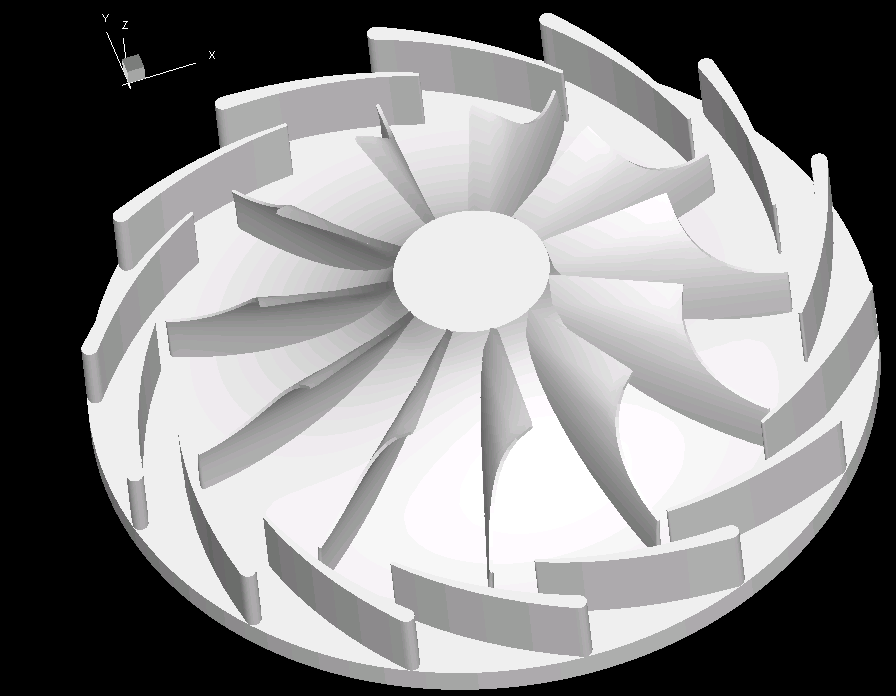
\includegraphics[width=0.5\textwidth]{./figures/3D_Geometry_NasaTurbine_fromAxcent_1.png}
  % \vskip-0.2cm
  \caption{Three-dimensional Geometry obtained with \textit{AxCent} from \textit{RITAL} one-dimensional preliminary design.}
  \label{fig_3D_geometry}
\end{figure}

Assuming periodicity, only one blade passage for each bladed segment was modelled. 
Meshes used for the calculations were generated with the \textit{AxCent} program using geometric parameters
imported from \textit{RITAL} and then exported as \textit{Fluent} mesh files.
Boundary conditions were based on the reported values for the design-point input conditions, 
specifically, the reported design point values for the mass flow rate, 
total temperature at the stator inlet and rotor outlet as well as static backpressure at the rotor outlet.
Density was calculated assuming an ideal gas behaviour and the transport properties for argon were calculated by the use of polynomial and Sutherland law approaches for thermal conductivity and viscosity respectively. 
As a first approach, the specific heat \textit{C$_p$} as well as the ratio of specific heats \textit{$\gamma$} were considered constants and equal to 520.3 J/(kg·K) and 5/3 respectively.

Variables such as static pressure, mass flow rate and velocities were also monitored during the calculations and the presented results were obtained when their variation at the inlet and outlet of both the stator and rotor was considered residual.

\clearpage

\subsection{Results}
\label{sec:kofsky_results}
%
\begin{figure}[htbp]
  \centering
  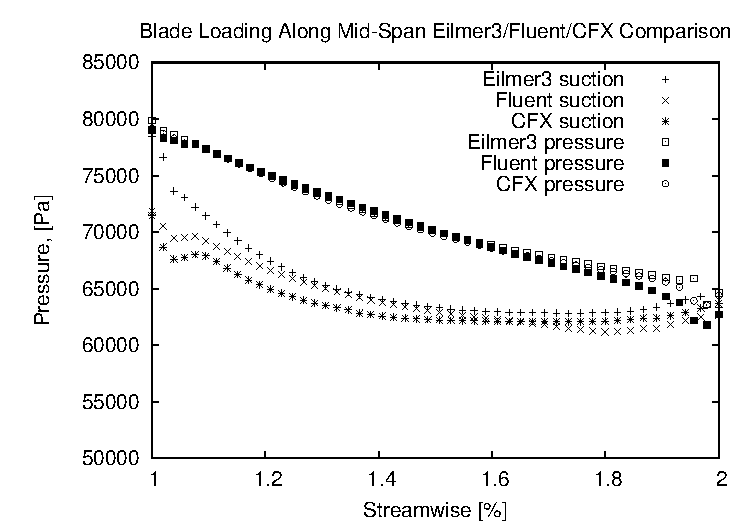
\includegraphics[width=0.60\linewidth]{./figures/Blade_Loading_Plot_Eilmer3_Fluent_CFX_Mesh_D.pdf}
  \vskip-0.2cm
  \caption{Comparison Between \textit{Eilmer3}, \textit{CFX} and \textit{Fluent} Considering Inviscid Flow.}
  \label{Comparison_Eilmer_Fluent}
\end{figure}

\cleardoublepage
%--------------------------------------------------------------------

\bibliographystyle{unsrt}
\bibliography{bibtex/pj,bibtex/eccomas,bibtex/upwind}

\cleardoublepage
\appendix

\section{UDF Boundary Conditions for the NASA Rotor}
\label{user-defined-bc-sec}\index{boundary condition}
%
\topbar
\lstinputlisting[language={}]{../3D/nasaRadialRotor/udf-rotor-periodic-bc.lua}
\bottombar \\


\cleardoublepage
\printindex
\end{document}
